    A primary concern in test is the limited resources available to test engineers. 
    These constraints severely limit the breadth of IC test. 
    Most circuits are only tested over a brief period of time or with limited computational resources. 
    Granted, if resources were unlimited we would want to test for every possible manufacturing defect.
    Unfortunately, resources are scarce in any industry, and especially so in the circuit design world. 
    Even with unlimited resources, if an average-sized circuit were tested for every possible fault, it could take longer than the known age of the universe to finish. 
    We would finally be able to present a tested product and then the universe would collapse on itself. 
    Because of these limitations, it becomes necessary to shrink the test space to a reasonable size. 
    The work detailed in this paper discusses how cell-aware test-space minimizing decisions can be made during functional simulation.


    Fault models are used as aids by test engineers to describe possible defects in a circuit and to generate input patterns to test for them. 
    One of the more predominantly used fault models is known as the ``Stuck-At Fault Model.''
    In this model, wires are modeled as being stuck at logic value-1 (\textit{shorted to $V_{dd}$}) or logic value-0 (\textit{shorted to ground}).
    One essential fact about this model, is that defects occur on the lines between gates,  not within them. 
    For example, to represent a potential stuck-at fault, the top wire in Figure \ref{fig:safault} is stuck-at 0 and is therefore \textit{modeled} as being grounded.

    \begin{figure}[h!]
        \begin{center}
            \caption{Example of Stuck-At Fault}
            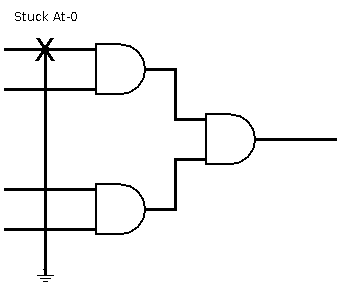
\includegraphics[scale=0.5]{Figures/sa0.png}
            \label{fig:safault}
        \end{center}
    \end{figure}

    This particular fault will cause major problems because the output of the circuit evaluates to 0 without regard to any other inputs. 
    Note that, in this case, the defect is described and conceptualized as a problem within the boundary between primary inputs and the gate, rather than occurring within the gate itself.


    To test for any fault you must first excite the fault and then observe the output.
    In this case we would need to make certain that the first PI (Primary Input) was set to 1 in order to excite the fault.
    We would also need to ensure that the fault will propagate to the output of the entire circuit. 
    For this particular fault, only one pattern will excite the fault and allow propagation to the output (\textit{inputs = 1111}). 
    Generally an ATPG (Automatic Test Pattern Generation) tool is used to create a list of possible patterns that could detect a fault.
    In this research we used both stuck-at fault ATPG and ATPG on a UDFM (User Defined Fault model, defining cell-aware type faults), by taking advantage of a built-in feature of Mentor Graphic's Tessent. 

    For the research in this paper, we consider a fault model known as the ``Cell-Aware Fault Model.''
    This fault model considers the transistor arrays within a logic gate and is explained in more detail with an example in section \ref{sec:caf}.
    The focus of this research is to determine a method for assigning an ``importance attribute'' to each of the cell-aware faults. 
    In other words, because we cannot focus on all potential cell-aware faults, how can we decide which ones present the most obvious flaws during normal usage? 
    To make this determination we propose using an attribute of a cell-aware fault called ``Mandatory Conditions'' during functional simulation to rank faults. 
    Functional simulation will be discussed in more detail in Section \ref{sec:fs}.
    The way that we performed functional simulation will be discussed in Section \ref{sec:meth}.
    Results and analysis will be discussed in Sections \ref{sec:res}.

\begin{comment}


    The abstract concept of a cell-aware fault is best described as any fault that is caused by a certain defect within a standard cell. Meaning that the fault specifically models a problem within the transistor array of the cell. Because this describes exactly every defect from manufacturing view, the fault model can be thought of more effectively as a model that represents faults that cannot be explained by some other traditional fault model such as the stuck at or bridging fault model. The cell-aware model and it's testing framework as well as ATPG methods were introduced by Hapke et al. \cite{5355741} \cite{Hapke} \cite{6401533}. The cell-aware fault model pays particular attention to the contents of the standard cell library which is used in the design of a circuit. The promise of using this fault model was explored in more detail by Rajski et al. \cite{5227030}. The effectiveness of the cell-aware fault model for detecting faults, and a comparison to the small delay defect fault model was explored by Fan Yang et al. \cite{6979084}. A case study regarding the usefulness of the cell-aware fault model on diagnosing a micro-controller was done by Prabhu et al. \cite{6847826}.

    In conjunction with the research discussed in this paper we discovered that n-detect for forcing multiple detections in certain ATPG schemes wouldn't work for cell-aware type faults. Consequently the definition of a cell-aware type fault in contrast to a pure cell-aware fault was discussed in a previous paper we wrote. \cite{6875445} The difference between what we have been referring to as a cell-aware type fault and a pure cell-aware fault arises in the derivation of each. As above mentioned, the cell-aware fault model can be viewed two ways that are essentially the same. The first is as an internal defect something tangible within the transistor array, Cell-aware faults can be derived by examining the electrical connections, and relationships. The second is as a fault that cannot be described by another fault model, and would thus not be tested for in ATPG targeting a specific type of fault. viewing the cell-aware fault by this second means is simply not the standard meaning for one, and we have hence taken to referring to them as cell-aware type faults. The definition of, and creation of the cell-aware type fault model is where the discussion of our methodology begins.

\end{comment}
